In the following test experiments we evaluate the benefits of passing additional information through the layers of the hypervisor and guests for profiling.  Unless otherwise noted, each experiment is performed on a \emph{Personal} and \emph{Business} scale virtualization platform (Table \ref{virtSize}).  Both systems have CentOS and Xen Server installed (Table \ref{softStack}) for the software stack installed.

\subsection{Verify Interference}
In this experiment we verify that our test framwork can generate a load that degrades the application when run with external interference.  There is a significant drop in performance from a single guest test to multiple guests running concurrently. Monitoring resources in only the guest domain provides little information about exteranl systems causing performance problems. 

To begin this exercise, we divide the physical memory and CPUs into four equal parts and create four individual guest virtual machines (Dom1 - Dom4).  
Each virtual machine is given 25\% of the available resources so that no guest virtual machine would interfere with another machine if they were on separate physical systems.  
We start only our Dom1 machine and run our experimental test with PGbench.  
On our \emph{Business} Dell server, Dom1 is allocated 2GB vRAM and 2 vCPU, while on our \emph{Personal} IBM server Dom1 is given 512MB vRAM and 1 vCPU.  

The test starts by initializing a very small database and runs PGBench and collect the TPS.  
Then we increase the DB size slightly and run the benchmark again.  
After repeating this process several times, we can see that when the DB size changes to an I/O bound system its performance drops significantly (Figure \ref{fig:smallIO}).  
This is due to the fact that it must fetch database rows from the disk and it is much slower.  

\begin{description}
  \item[Small DB] The working set can fit into main memory.  Performance is based on memory.
  \item[Medium DB] The working set is swapped to disk occasionally. Performance is moving from memory to I/O.
  \item[Large DB] Most reads need to go to disk.  Performance is based on Disk I/O.
\end{description}

% Section 7.1.2
\subsubsection{With Interference}
Then we create external machine interference by running Dom1 concurrently with Dom2, Dom3, and Dom4. Each of the Dom2 - Dom4 systems are configured the same as Dom1.  We create a 2 GB database on each guest of the Dell, and a 1GB database on each guest of the IBM.  We run a PGBench in a loop to continuously create I/O interference on each external guest machine (Dom2 - Dom4). Concurrently we run our benchmark, and collect performance statistics only from Dom-1.  When the system is not I/O bound (Small DB) there is about a 28\% drop in performance (4434 TPS - 3208 TPS) on the IBM server and little change in the Dell server (Table \ref{fig:tps1}).  On both servers the guest becomes an I/O bound system quicker with external interference.

\begin{table}[h]
\begingroup
    \fontsize{10pt}{12pt}\selectfont
\begin{subtable}[h]{0.45\textwidth}
  \begin{tabular}{ l | r | r | r }
    DB Size & Single & Interfernce & Drop \\
    \hline
    Small & 4434 & 3208 & 28\% \\ \hline
    Medium & 2149 & 216 & 90\% \\ \hline
    Large & 260 & 197 & 24\% \\  \hline
    \hline
  \end{tabular}
\caption{IBM x3650 with 2GB RAM:  Each Guest domain has 512MB Allocated.}
\end{subtable}
\hfill
\begin{subtable}[h]{0.45\textwidth}
  \begin{tabular}{ l | r | r | r }
    DB Size & Single & Interference & Drop \\
    \hline
    Small & 5772 & 5734 & 0.7\% \\ \hline
    Medium & 1608 & 162 & 90\% \\ \hline
    Large & 359 & 82 & 77\% \\  \hline
    \hline
  \end{tabular}
\caption{Dell T410 with 12GB RAM:  Each Guest domain has 2GB Allocated. }
\end{subtable}
\caption{Dom1 TPS difference from interference for 3 database sizes.}
\label{fig:tps1}
\endgroup
\end{table}

% Section 7.1.3
\begin{figure}[!h]
  \begin{center}
  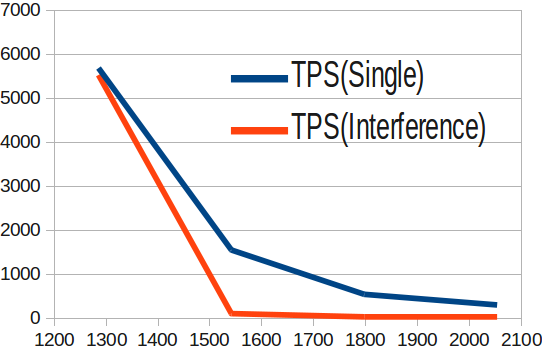
\includegraphics[width=4in]{images/MedScale.png}
  \caption{TPS with and without interference.  Moving from a Medium DB to a Large DB.}
  \label{fig:smallIO}
  \end{center}
\end{figure}

Trying to analyze the performance drop in Dom1 without knowing about this external interference is difficult.  There were no changes to Dom1 when run by itself and run with other guests.  By using the system \emph{sar} utility we can examine available memory, SwapIn and BytesIn/s to see if we can determine why the application benchmark is degraded without collecting external information (Figure \ref{fig:vmstat}).  Memory is not used as efficiently, the system almost completely elimiates swapping data in, and also can't read as quickly from disk.  However, there is no indication that the problem was due to an external guest and hypervisor using those resources.  A DBA looking at these numbers may conclude that kernel swap or DB tuning may fix the problem.  
The root cause of the performance drop is due to external interference, which is not known from examining the data available.

\begin{table}[h]
  \begin{tabular}{ l | r | r | r }
    VMstat & Single & Multiple & Drop \\ \hline
	SwapIn/s & 1,480 & 85 & 94\% \\
	BytesIn/s & 6,877 & 4,438 & 35\% \\
	CPU IOwait & 92\% & 93\% & 1\% \\
  \end{tabular}
\caption{IBM x3650.  Some resource statistics collected with vmstat on Dom1 with a Large database while running alone and with multiple systems.} 
\label{fig:vmstat}
\end{table}

% Section 7.2
\subsection{Personal Server}
In the previous experiment we showed the interference that can occur when external I/O interference is applied to a guest domain, and only looking at the virtual resources in the domain does not indicate the problem.  In this experiment, we verify our design to show interference from external systems, when the system is I/O bound.  The results are from our IBM x3650, where each guest is configured to use 512MB of vRAM.  First, we run the benchmark with a 640MB database without interference and calcuate the overhead.  Then we start Dom2 - Dom4, run the benchmark in Dom1, and calculate the interference.  We compare the results of the calculated interference with the performance drop in the application.

\begin{Verbatim}
# xm list
Name                            ID   Mem VCPUs      State   Time(s)
Domain-0                        0  1988     4     r-----  88871.2
Test_VM1                        1   512     1     -b----  60187.0
Test_VM2                        2   512     1     -b----   5722.0
Test_VM3                        3   512     1     -b----   5273.0
Test_VM4                        4   512     1     -b----   5203.5
\end{Verbatim}

% Section 7.2.1
\subsubsection{Overhead}
We calculate the overhead for the guest OS paging and the I/O reads using the resource counters defined in our design.  While calculating the overhead we also collected the application performance at 415 TPS without any external interfernece.

% See Test7_1Results.xls (Barbaro - Exp7.2(P2))
\begin{table}[h]
\begin{tabular}{ l l l p{5cm} }
  Counter     & Dom0 & Dom1 & $Overhead_V$ \\
  \hline
	pgpgin    & 332,504 & 165,901  &  \\
	pgfault   &  25,648 & 132,691  & \\
	r sectors & 332,504 & 331,803  &\\
	r\_ms     &  63,356 &  72,428  & \\
	r total   &  11,145 &  12,166  & \\
    \textbf{reads/s}    & 637 & 767 & \\
    \textbf{AvgRdWait}  & 3.59 & 3.70 & 2.9\% \\ 
  \hline
\end{tabular}
\caption{Overhead on the IBM x3650.}
\label{tab:OverheadSmall}
\end{table}

One thing to notice is that the pgpgin from the Dom1 is about half of the host in Dom0.  
We also see in Dom0 that pgpgin is exactly the same as the sectors read.  
After some research on this we believe that the Dom0 and guest kernels are reporting different units of measurements, and there is not really 2x overhead for the pgpgin statistic.  
In the Linux 2.4 and later kernel blocks and sectors were both 512 bytes, and the unit of measurement for pages in were reported in 1K sizes.  Since the Dom0 kernel is version 3.4.54 and the guest kernel is 2.6.32, we believe that the guest is reporting 1KB pages, and the Dom0 is reporting 512 byte pages to match the sector (and block) size.  In order to report an accurate results, we would need to ensure that the unit of measurement for values reported between the guest and hypervisor are consistent.  

% Section 7.2.2 - Test7_1Resultx.xls (Barabaro- Exp7.2(P2))
\subsubsection{Memory Interference}
We repeat the previous experiment with 4 guest domains all running at the same time.  Since the DB size in Dom1 is 640MB and there is 512MB of vRAM on Dom1, we can say that Dom1 is bound by disk I/O speed.  We run the experiments with the other 3 guest domains running a memory bound database.  
We create a Small DB of 128MB in each of the external domains to generate memory interference on Dom1.

\begin{table}[h]
\begin{tabular}{ l l l l p{5cm} }
  Counter & Dom0 & Dom1 & $Interference_{RPS}$ \\
  \hline
	pgpgin    & 328,144 & 128,176 &  \\
	pgfault   &  57,293 &  95,591 &  \\
	r sectors & 328,144 & 256,352 &  \\
	r ms      & 103,483 &  70,751 &  \\
	r total   &  13,365 &   9,547 &  \\
    \textbf{reads/s}    & 446 & 318 & 28.6\%  \\
    \textbf{AvgRdWait}  & 7.74 & 7.41 & \\ 
  \hline
\end{tabular}
\caption{Interference calculated from Small 128MB DB in Dom2 - Dom4.  TPS dropped by 20\%} 
\label{fig:InterferenceSm}
\end{table}
We calculate the increased wait time using the $AvgRdWait$ we collected previously. We calculate $Interference_{ARW} = 56\%$  Since this is greater than the interference from througput we calculate the $Interference_{EXT} = 28.6\%$.

From these tests, Dom1 had 331 TPS, and was degraded from 415 TPS, a performance drop in the application of 20\%.  It is not shown in these results, but Dom2 - Dom4 was able to cache the entire working set in memory and did not issue any read requests.  Dom1 was the only domain to issue read request. The totals from all guests domains for each of the three read counters is exactly the same as Dom1.  

% Section 7.2.3 - Test7_1Resultx.xls (Barabaro- Exp7.2(P2))
\subsubsection{I/O Interference}
Now we create I/O Interference in the three guest domains by creating a 640MB Large DB in Dom2 - Dom4.  Since each guest has 512MB vRAM, this should cause significant I/O contention in Dom1.

\begin{table}[h]
\begin{tabular}{ l l l l p{5cm} }
  Counter     & Dom0    & Dom1    & $Interference_RPS$ \\
  \hline
	pgpgin    & 549,419 & 97,092 &  \\
	pgfault   &  58,201 & 86,765 &  \\
	r sectors & 549,419 &194,163 &  \\
	r ms      & 285,334 & 71,585 &  \\
	r total   &  20,723 &  7,259 &  \\
    \textbf{reads/s}    & 691 & 242 &   65\% \\
    \textbf{AvgRdWait}  & 13.8 & 9.86 &  \\ 
  \hline
\end{tabular}
\caption{Interference calculated Large 640MB DB in Dom2 - Dom4.  TPS dropped by 39\%}
\label{fig:InterferenceLg}
\end{table}
We calculate $Interference_{ARW} = 74\%$  Since this is greater than the interference from througput we calculate the $Interference_{EXT} = 65\%$.

During these tests, the application benchmark in Dom1 decreased to 254 TPS.  This is much less than when run without interference (415 TPS) and with memory interference (331 TPS).  All of the read counters showed significant interference.  Additionally we are showing some interference from page faults.  

\subsection{Business Server}
For this experiment we use our Dell server with 12GB of physical RAM. We configure all Dom1 to use 4GB of vRAM and configure Dom2 - Dom4 as noted below.  We assign some different CPUs to the guest machines. We create a medium database of 3.2GB in Dom1.   And create Medium and Large databases in the external guest domains to change the different workloads in the guests.

\begin{Verbatim}
Name                       ID   Mem VCPUs      State   Time(s)
Domain-0                    0   872    16     r-----  27116.4
TestVM1                     1  4096     1     -b----   1127.7
TestVM2                     2  3072     2     -b----   1735.8
TestVM3                     3  2048     1     -b----   1588.1
TestVM4                     4  2048     2     -b----   1906.1
\end{Verbatim}

\subsubsection{Overhead}
We calculate the $Overhead_V$ in Dom1 using the same method as described previously (Table \ref{tab:OverheadBus}).  We can see that the overhead from virtualization on this platform (2.9\%) is about the same as the overhead on the previous serer even though the wait time was increased significantly.  We also see that our reads/s was decreased, but our datase throghput was faster at 1,348 TPS.  This is because in this server the database size is smaller than the available memory.

\begin{table}[h]
\begin{tabular}{ l l l p{5cm} }
  Counter     & Dom0 & Dom1 & $Overhead_V$ \\
  \hline
    \textbf{reads/s}    & 275  & 281 & \\
    \textbf{AvgRdWait}  & 14.0 & 13.6 & 2.9\% \\ 
  \hline
\end{tabular}
\caption{Overhead on the IBM x3650.}
\label{tab:OverheadBus}
\end{table}

\subsubsection{Interference}
% See WallEve_4_16_14.txt 
In the previous experiment for calculating interference we used 3 external guest domains, and changed the workload in the guest domains.  In this experiment, we create interference using 1 external domain at a time.  The first result is the same as the overhead calculation above.  This is a single guest domain Dom1 without external interference.  Then we run Dom1 with Dom2 and calculate the interference with a single external domain.  We continue to add domains and calculate the interference and application performance drop in TPS (Table \ref{tab:domains}).

\begin{table}[!h]
\begin{tabular}{ l l l l l l p{9cm} }
                   & TPS   & reads/s & reads/s & AvgRdWait & $Interference_{RPS}$ & $Inteference_{AWR}$ \\
	Experiment     & Dom 1 & Dom0     & Dom1     & Dom0      & $Interference_{EXT}$ &             \\
	\hline
    Dom1 (Only)     & 1348 & 275      & 281      & 14.0     &  -2.1\%  &   0.0\%   \\
    Dom1 + 1 guest  &  703 & 214      & 137      & 33.2     &  36.0\%  &   61.1\%  \\
    Dom1 + 2 guests &  543 & 246      & 108      & 44.0      &  56.1\%  &   75\%    \\
    Dom1 + 3 guests &  378 & 259      &  76      & 59.5    &  70.7\%  &   80.2\%  \\
\end{tabular}
\caption{Interference generated from 1, 2, and 3 external guest domains.}
\label{tab:domains}
\end{table}

From this we can see that as more external domains are added, our test benchmark degrades as expected.  We are also able to measure the interference which increases as more domains are added.  This is critical information to guest domains when they are experiencing performance problems and can quickly identify the root cause of problems for I/O.

% Section 7.5
\subsection{Verification without interference}
In the previous two experiments, we showed how our method can give a guest domain vital information when it is degraded from external interference.  However, what if the guest domain was degraded due to an application bug, DB change, or misconfiguration?   In that case we want our method to show that there is not any external interference.

We have previously demonstrated that the database TPS can become degraded as the size of the database increases.  Now we show that by simply increasing the I/O load from a single domain, that our method does not report external interfernce. In this case the application is degraded because the working set exceeds the available memory. We also change the number of DB connections to change the read wait time.  The application depends on the I/O system for performance, but it is not degraded from external interference.

% See Test7_1Results.xls - Barbaro Exp7.2 and Barbaro_Dom29.txt
\begin{table}[h]
\begingroup
    \fontsize{10pt}{12pt}\selectfont
\begin{tabular}{ l l l l l l p{9cm} }
                   & reads/s & reads/s & AvgRdWait & $Interference_{RPS}$ & $Inteference_{AWR}$ \\
	Experiment     & Dom0     & Dom1     & Dom0      & $Interference_{EXT}$ &             \\

    Test & Guest & Hypervisor  & $Interference_{RPS}$ \\
    \hline
    Baseline                   & 372 & 406 & 5.7 & -6\% & 0.0\%   \\  %Test 1
    Increase DB size           & 538 & 563 & 7.8 & -6\% & 26.9\% \\  %Test 3
    Increase DB Connections    & 836 & 875 &15.4 & -5\% & 63.0\% \\  %Test 4
	Decrease DB Connections    & 279 & 144 & 4.7 & 48\% & -17\%  \\  %Test 5
    With 3 ext domains         & 691 & 242 &13.8 & 65\% & 59.0\% \\  % From above
    \hline
  \end{tabular}
\caption{Tests without interference, our method does not report interference. }
\label{tab:HypervisorGuest}
\endgroup
\end{table}

One interesting result is that when we decreased the number of DB connections, we experienced a significant increase in reads in the hypervisor.  We ran this experiment several times, and verified that this was accurate.  For some reason the hypervisor increased the reads (since there were not any external domains).  Since our calculation determines interference from external domains, it did not show interference because there was no increase in the wait time.

By analyzing the throughput from both the guest layer and hypervisor layer, we can see that our method reports interference only when external interference is applied to the guest domain.  When we showed the guest view (Table \ref{tab:guestOnly}) it was difficult to determine if the problem was from a change in the guest application or an external domain.  With these tests we can see that we need to have both an increase in wait time in the hypervisor as well as additional throughput from external domains.


\subsection{Results Analysis}
We completed several different experiments on two different virtualization platforms.  In section 7.1 we verified our test method and showed how performance can decrease without interference by increasing the size of the database.  We also showed that for each database size when external guest domains run concurrently they cause interference and degrade the guest application.  In section 7.2 we looked at our \emph{Personal} size server which had 2 GB ram and 4 CPUs.  We were able to calcuate the interference from external domains that only used memory, and external domains that were also I/O bound.  Our calculations for interference changed at the same rate of application degredation.  In section 7.3 we used our \emph{Business} server and calculated the overhead and interference from virtualization.  We created external interference from different numbers of guest domains, and found as more external guests are added our calculated interference increases at the same rate as the application performance decreases.  Finally, in section 7.5 we validated that when the application degrades due to internal changes, our method does not report it as external interference from virtualization.

